%
% ---------------------------------------------------------------
% Copyright (C) 2012-2018 Gang Li
% ---------------------------------------------------------------
%
% This work is the default powerdot-tuliplab style test file and may be
% distributed and/or modified under the conditions of the LaTeX Project Public
% License, either version 1.3 of this license or (at your option) any later
% version. The latest version of this license is in
% http://www.latex-project.org/lppl.txt and version 1.3 or later is part of all
% distributions of LaTeX version 2003/12/01 or later.
%
% This work has the LPPL maintenance status "maintained".
%
% This Current Maintainer of this work is Gang Li.
%
%

\documentclass[
 size=14pt,
 paper=smartboard,  %a4paper, smartboard, screen
 mode=present, 		%present, handout, print
 display=slides, 	% slidesnotes, notes, slides
 style=tuliplab,  	% TULIP Lab style
 pauseslide,
 fleqn,leqno]{powerdot}


\usepackage{cancel}
\usepackage{caption}
\usepackage{stackengine}
\usepackage{smartdiagram}
\usepackage{attrib}
\usepackage{amssymb}
\usepackage{amsmath} 
\usepackage{amsthm} 
\usepackage{mathtools}
\usepackage{rotating}
\usepackage{graphicx}
\usepackage{boxedminipage}
\usepackage{rotate}
\usepackage{calc}
\usepackage[absolute]{textpos}
\usepackage{psfrag,overpic}
\usepackage{fouriernc}
\usepackage{pstricks,pst-3d,pst-grad,pstricks-add,pst-text,pst-node,pst-tree}
\usepackage{moreverb,epsfig,subfigure}
\usepackage{color}
\usepackage{booktabs}
\usepackage{etex}
\usepackage{breqn}
\usepackage{multirow}
\usepackage{natbib}
\usepackage{bibentry}
\usepackage{gitinfo2}
\usepackage{siunitx}
\usepackage{nicefrac}
%\usepackage{geometry}
%\geometry{verbose,letterpaper}
\usepackage{media9}
\usepackage{animate}
%\usepackage{movie15}
\usepackage{auto-pst-pdf}

\usepackage{breakurl}
\usepackage{fontawesome}
\usepackage{xcolor}
\usepackage{multicol}



\usepackage{verbatim}
\usepackage[utf8]{inputenc}
\usepackage{dtk-logos}
\usepackage{tikz}
\usepackage{adigraph}
%\usepackage{tkz-graph}
\usepackage{hyperref}
%\usepackage{ulem}
\usepackage{pgfplots}
\usepackage{verbatim}
\usepackage{fontawesome}


\usepackage{todonotes}
% \usepackage{pst-rel-points}
\usepackage{animate}
\usepackage{fontawesome}

\usepackage{listings}
\lstset{frameround=fttt,
frame=trBL,
stringstyle=\ttfamily,
backgroundcolor=\color{yellow!20},
basicstyle=\footnotesize\ttfamily}
\lstnewenvironment{code}{
\lstset{frame=single,escapeinside=`',
backgroundcolor=\color{yellow!20},
basicstyle=\footnotesize\ttfamily}
}{}


\usepackage{hyperref}
\hypersetup{ % TODO: PDF meta Data
  pdftitle={Presentation Title},
  pdfauthor={Gang Li},
  pdfpagemode={FullScreen},
  pdfborder={0 0 0}
}


% \usepackage{auto-pst-pdf}
% package to show source code

\definecolor{LightGray}{rgb}{0.9,0.9,0.9}
\newlength{\pixel}\setlength\pixel{0.000714285714\slidewidth}
\setlength{\TPHorizModule}{\slidewidth}
\setlength{\TPVertModule}{\slideheight}
\newcommand\highlight[1]{\fbox{#1}}
\newcommand\icite[1]{{\footnotesize [#1]}}

\newcommand\twotonebox[2]{\fcolorbox{pdcolor2}{pdcolor2}
{#1\vphantom{#2}}\fcolorbox{pdcolor2}{white}{#2\vphantom{#1}}}
\newcommand\twotoneboxo[2]{\fcolorbox{pdcolor2}{pdcolor2}
{#1}\fcolorbox{pdcolor2}{white}{#2}}
\newcommand\vpspace[1]{\vphantom{\vspace{#1}}}
\newcommand\hpspace[1]{\hphantom{\hspace{#1}}}
\newcommand\COMMENT[1]{}

\newcommand\placepos[3]{\hbox to\z@{\kern#1
        \raisebox{-#2}[\z@][\z@]{#3}\hss}\ignorespaces}

\renewcommand{\baselinestretch}{1.2}


\newcommand{\draftnote}[3]{
	\todo[author=#2,color=#1!30,size=\footnotesize]{\textsf{#3}}	}
% TODO: add yourself here:
%
\newcommand{\gangli}[1]{\draftnote{blue}{GLi:}{#1}}
\newcommand{\shaoni}[1]{\draftnote{green}{sn:}{#1}}
\newcommand{\gliMarker}
	{\todo[author=GLi,size=\tiny,inline,color=blue!40]
	{Gang Li has worked up to here.}}
\newcommand{\snMarker}
	{\todo[author=Sn,size=\tiny,inline,color=green!40]
	{Shaoni has worked up to here.}}

%%%%%%%%%%%%%%%%%%%%%%%%%%%%%%%%%%%%%%%%%%%%%%%%%%%%%%%%%%%%%%%%%%%%%%%%
% title
% TODO: Customize to your Own Title, Name, Address
%
\title{San Francisco Crime classification}
\author{
Jia Huang
\\
\\Xi'an Shiyou University
%\\Deakin University
\\Chinese Academy of Sciences
%\\ \today
}
%\date{\gitCommitterDate}


% Customize the setting of slides
\pdsetup{
% TODO: Customize the left footer, and right footer
rf=\href{http://www.tulip.org.au}{
Last Changed by: \textsc{\gitCommitterName}\ \gitVtagn-\gitAbbrevHash\ (\gitAuthorDate)
},
cf={San Francisco Crime classification},
}


\begin{document}

\maketitle

%\begin{slide}{Overview}
%\tableofcontents[content=sections]
%\end{slide}


%%==========================================================================================
%%
\begin{slide}[toc=,bm=]{Overview}
\tableofcontents[content=currentsection,type=1]
\end{slide}
%%
%%==========================================================================================


\section{Project Overview}


%%==========================================================================================
%%
\begin{slide}{Project Background And Purpose}
\begin{center}
\twotonebox{\rotatebox{95}{Defn}}{\parbox{.89\textwidth}
{
\begin{itemize}
\item Background
\\From 1934 to 1963, San Francisco was infamous for housing
some of the world's most notorious criminals on the 
inescapable island of Alcatraz. Today, the city is known
more for its tech scene than its criminal past. But, with 
rising wealth inequality, housing shortages, and a proliferation
of expensive digital toys riding BART to work, there is no 
scarcity of crime in the city by the bay. From Sunset to SOMA, 
and Marina to Excelsior, this dataset provides nearly 12 years
of crime reports from across all of San Francisco's neighborhoods.
~\\
\item Purpose
\\predict the category of crime that occurred, given the time 
and location visualize the city and crimes (see Mapping and 
Visualizing Violent Crime for inspiration) Content.
\end{itemize}
}}

\end{center}
\bigskip
\begin{center}
\begin{tabular}{c| c c c c }
\toprule
\midrule

\bottomrule
\end{tabular}
\end{center}
\bigskip

%%==========================================================================================
\begin{note}
First, I will introduce the problem definition.
In the real life,
a teacher may be interested in the characteristics that
make one student obvious different from others.
Or,
NBA sports coaches would prefer to
know the advantages and disadvantages of one player.
Here, the player can be regarded as a query object.

For example, team A has five players,
each player has four features.
The NBA sports coaches may want to know the features of
player $1$ that are different from others.

The above example can be seen as outlying aspects mining.
The main purpose of outlying aspects mining is to identify
the outstanding features of the query object.
\end{note}
%%==========================================================================================

\end{slide}
%%
%%==========================================================================================


%%
%%==========================================================================================


\section{Data Pre-Processing}


%%==========================================================================================
%%
\begin{slide}{Feature Item}
%Related Work - Outlying Aspects Mining
This dataset contains incidents derived from 
SFPD Crime Incident Reporting system. The data 
ranges from 1/1/2003 to 5/13/2015. The training 
set and test set rotate every week, meaning 
week 1,3,5,7... belong to test set, week 2,4,6,8 
belong to training set. There are 9 variables:


\bigskip
~\\
\twocolumn[
\savevalue{lfrheight}=5.6cm,
\savevalue{lfrprop}={
linestyle=solid,framearc=.2,linewidth=2pt},
rfrheight=\usevalue{lfrheight},
rfrprop=\usevalue{lfrprop}
]{
\begin{itemize}
  \item Characteristic Term
\begin{itemize}
\item
\smallskip
Dates 
\smallskip
\item 
\smallskip
Category 
\smallskip
\item
\smallskip
Descript
\smallskip
\item
\smallskip
DayOfWeek
\end{itemize}
\end{itemize} 
}{
  \begin{itemize}
    \item Characteristic Term
\begin{itemize}
\item 
\smallskip
PdDistrict
\smallskip
\item 
\smallskip
Resolution 
\smallskip
\item 
\smallskip
Address
\smallskip
\item 
\smallskip
X 
\smallskip
\item 
\smallskip
Y
\end{itemize}
\end{itemize}
}




%%==========================================================================================
\begin{note}
Let me introduce two existing methods:
Feature selection and score-and-search.

For feature selection,
the query point can be regarded as positive class and
the rest of the data can be regarded as negative class,
selected the features that best distinguish the two classes.

The advantages of this method are easy to operate,
and it's able to resolve dimensionality bias.
However, it has some drawbacks.
Firstly,
positive and negative classes are Not balanced,
secondly,
it can't quantify the outlying degree correctly.
Most importantly,
it doesn't identify group outlying aspects.
\end{note}
%%==========================================================================================

\end{slide}
%%
%%==========================================================================================

%%
%%==========================================================================================
\begin{slide}{Feature Item}
By making a comprehensive analysis of the nine
characteristic items in the data set mentioned 
above,we can reach the following conclusions:


\bigskip

\begin{figure}[htbp]
  \centering
  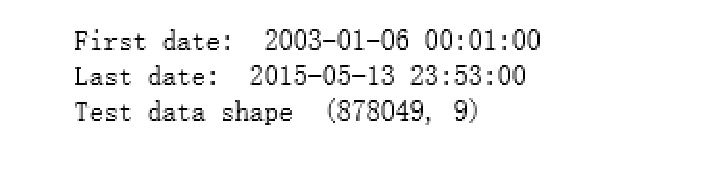
\includegraphics[width=1\textwidth]{kaggle/1.eps}
  \caption{}
\end{figure}
\setlength{\parindent}{2em}The data range was from 1/1/2003 to 5/13/2015, and 
a data training set containing nine feature items and 87,8049 
samples was created.
\end{slide}

%%
%%==========================================================================================

%%
%%==========================================================================================

\section{Feature Analysis}

%%==========================================================================================
%%

%%
%%===========================================================================================



%%
%%=============================================================================================
\begin{slide}[toc=,bm=]{}
\begin{itemize}
\item Statistics Were Made By Type Of 'Year' And 'Month'
\\Based on a comprehensive analysis of the data set provided by Kaggle's website,
it is clear that there are fewer crimes in summer and winter than in spring 
and fall.Therefore, a "seasonal" feature column can be added to the feature analysis.
\item 
By 'DayOfWeek' And 'Hour' Type
\\Friday saw the highest number of crimes, probably because of the American tradition 
of Friday parties.Sunday has the lowest crime rate.So you can add the "weekend or not" feature
column.Crime was lowest in the early hours of the morning and highest at 12 o 'clock and 17 and
18 o 'clock in the evening.Therefore, the time zone can be divided and the "time zone" feature 
column can be added
\end{itemize}

%%==========================================================================================
\begin{note}
In conclusion,
we firstly formalized the problem of
group outlying aspects mining,

Then proposed a novel method GOAM algorithm to address the problem of
group outlying aspects mining,
and the proposed method use pruning to reduce time complexity
while identifying the suitable set of outlying features for the interested group.

Thank you and any question?
\end{note}
%%==========================================================================================

\end{slide}
%%
%%==========================================================================================


%%
%%===========================================================================================

\section{Feature Selection} 

%%===========================================================================================
%%

\section{Modelling}

%%
%%============================================================================================

%%
%%==============================================================================================
\begin{slide}{Calculate the Baseline Value For The Model}
  Since this is a typical multi-classification problem, we 
  can choose to use many kinds of algorithms, including naive
   Bayes, KNN, decision tree and random forest.
\end{slide}

%%
%%===============================================================================================


\section{Model Optimization}

%%==========================================================================================
%%


\section{Ideas Improvement}

% TODO: Contact Page

\end{document}

\endinput
